\documentclass[dvipsnames]{beamer}
\input{mybeamerdefs}
\title{MRI Simulator Notes}
\author{Liam}
\date{\today}

\begin{document}

\begin{frame}
\maketitle
\end{frame}

\begin{frame}{Tasks}
\begin{itemize}
\item I computed the required parameters for the proper FOV and pixel size for the simulation.
\item I ran the excitation simulation of 2019-12-04 on Supershop and tracked the resource usage.
\item I wrote more code for the 2DFT simulation.
\end{itemize}
\end{frame}

\section{Parameter requirements}

\begin{frame}{Summary}
\begin{itemize}
\item The ems are arranged in a grid, with the number of grid points in each dimension being $2r_{\rm grid}+1$, with $r_{\rm grid}$ an integer.
\item The ems are placed at $x = [-x_{\rm lim}: \Delta x: x_{\rm lim}]$, where $\Delta x = x_{\rm lim}/r_{\rm grid}$ and similarly for $y$.
\item The number of samples of k-space taken in the phase-encoding direction ($y$) is $2r_{\rm pe}+1$ and the number of samples taken in the frequency-encoding direction ($x$) is $2r_{\rm fe}+1$, with $r_{\rm pe}$ and $r_{\rm fe}$ integers.
\item We require the field-of-view to satisfy $FOV_x \geq 2x_{\rm lim}$ and $FOV_y \geq 2y_{\rm lim}$.
\item We require a pixel dimension of $\Delta x \times \Delta y$.
\end{itemize}
\end{frame}

\begin{frame}
\begin{itemize}
\item For the field-of-view requirements, we use
\begin{equation*}
FOV_x = \frac{1}{\Delta k_x}\,,
\end{equation*}
where $\Delta k_x$ is the spacing between k-space samples in the $x$ direction, and similarly for $y$.
\item For the pixel size requirements, we use
\begin{equation*}
\delta_x \approx \frac{1}{2k_{x,max}}\,,
\end{equation*}
where $\delta_x$ is the spatial resolution in $x$ and $k_{x,max}$ is the maximum sample of k-space in the $x$ direction, and similarly for $y$.
\end{itemize}
\end{frame}

\begin{frame}
For the FOV requirements, I find
\begin{equation*}
\frac{r_{\rm fe}}{k_{x,max}} \geq 2x_{\rm lim}\,, \quad \frac{r_{\rm pe}}{k_{y,max}} \geq 2y_{\rm lim}\,.
\end{equation*}
For the pixel size requirements, I find
\begin{equation*}
\frac{x_{\rm lim}}{r_{\rm grid}} = \frac{1}{2k_{x,max}}\,, \quad \frac{y_{\rm lim}}{r_{\rm grid}} = \frac{1}{2k_{y,max}}\,.
\end{equation*}
\end{frame}

\section{Resource usage on Supershop}

\begin{frame}{Summary}
\begin{itemize}
\item The memory usage as a function of the number of ems is shown on the following slide for 1000, 2000, 5000, 10000 ems.
\item The maximum CPU usage from \texttt{top} that I observed was 969\% for $10^9$ ems (I did not run the simulation to completion). I suppose this means Python is using multiple cores automatically?
\end{itemize}
\end{frame}

\begin{frame}
\begin{center}
\includegraphics[height=0.8\textheight]{{supershop_resource_usage}}

1.8 kB per em
\end{center}
\end{frame}

\section{2DFT simulation}

\begin{frame}{Summary}
\begin{itemize}
\item I simulated a 2DFT pulse sequence with ems distributed as shown in the next slide.
\item The reconstruction is the slide following.
\end{itemize}
\end{frame}

\begin{frame}{Distribution of ems}
\begin{center}
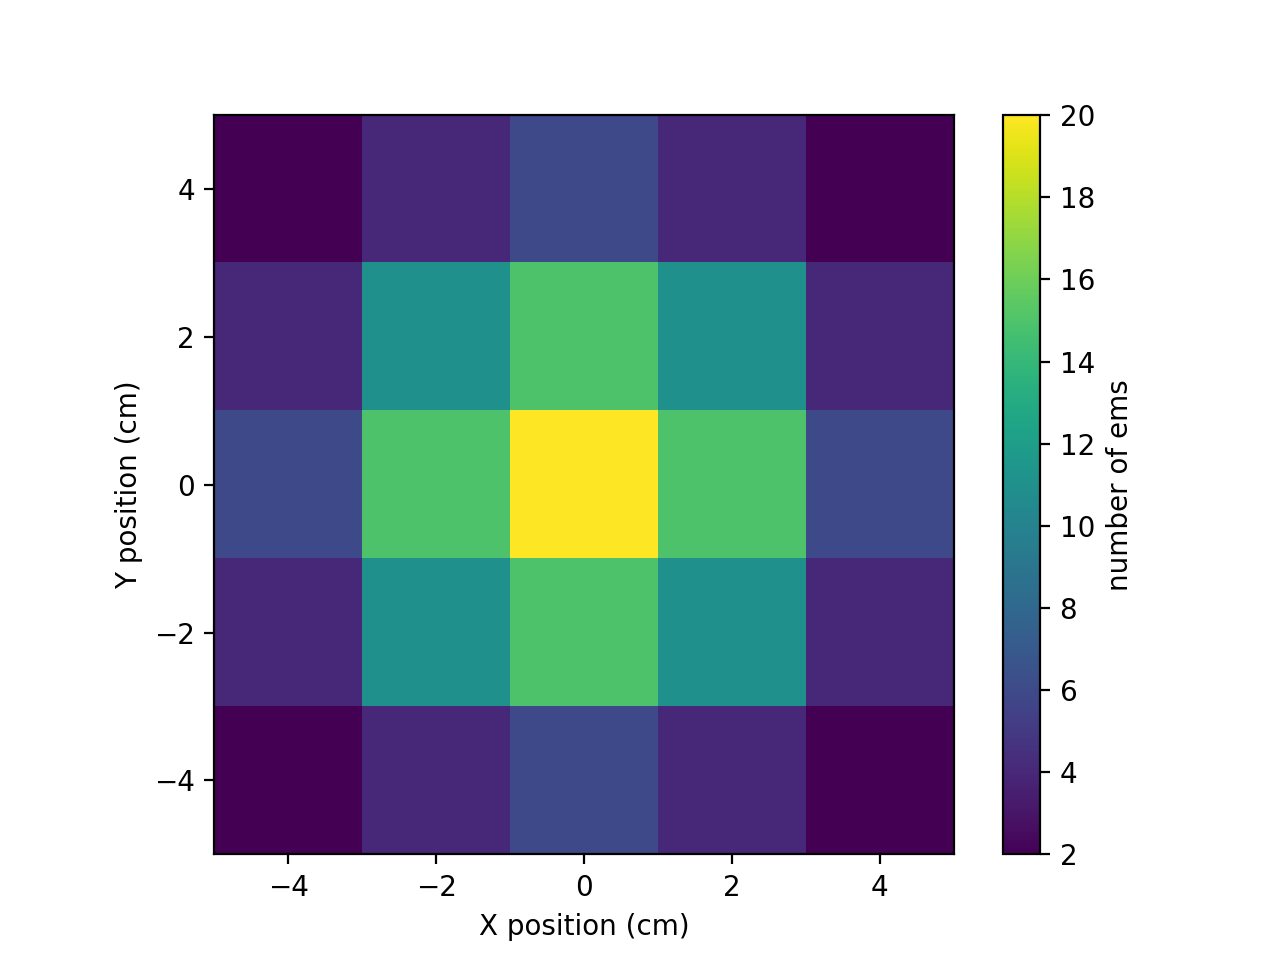
\includegraphics[height=0.8\textheight]{dist}
\end{center}
\end{frame}

\begin{frame}{Reconstruction}
\begin{center}
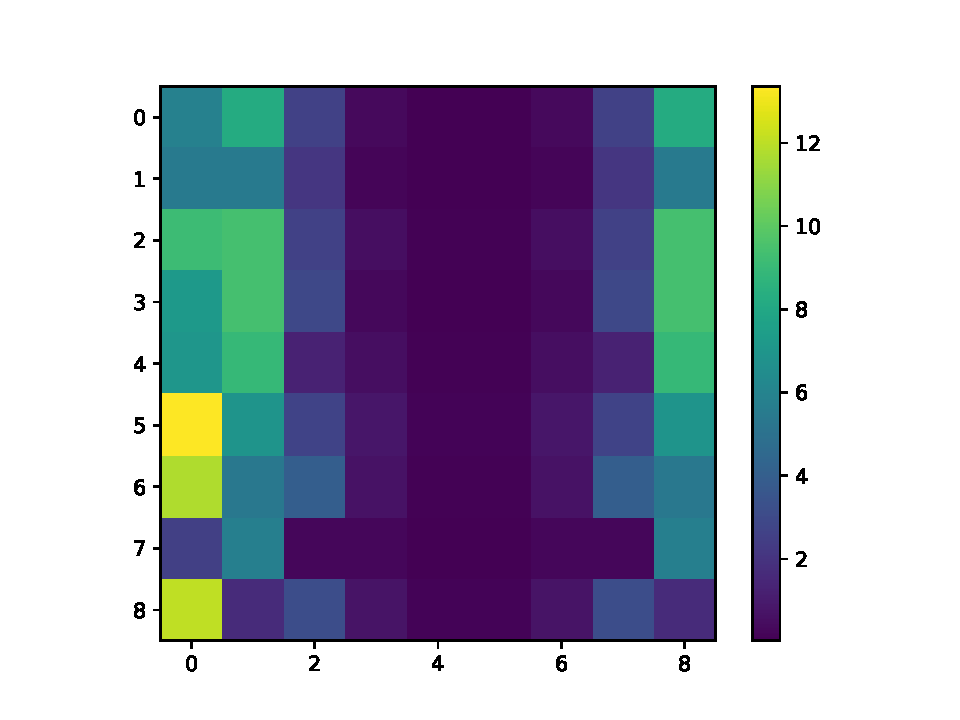
\includegraphics[height=0.8\textheight]{reconstruction}
\end{center}
\end{frame}

\begin{frame}{Comments}
\begin{itemize}
\item It looks like the reconstruction has a spatial shift.
\item The intensity values don't look quite right either.
\end{itemize}
\end{frame}

\end{document}